\documentclass[paper=a4, fontsize=11pt]{scrartcl}
\usepackage[T1]{fontenc}
\usepackage{fourier}
\usepackage[english]{babel}
\usepackage[protrusion=true,expansion=true]{microtype}	
\usepackage{amsmath,amsfonts,amsthm} % Math packages
\usepackage[pdftex]{graphicx}	
\usepackage{url}
\usepackage[style=authoryear-icomp,sorting=anyt]{biblatex}
\addbibresource{sample.bib}
\usepackage{float}
\usepackage{sectsty}
\allsectionsfont{\centering \normalfont\scshape}
\usepackage{fancyhdr}
\pagestyle{fancyplain}
\fancyhead{}										% No page header
\fancyfoot[L]{}											% Empty 
\fancyfoot[C]{}											% Empty
\fancyfoot[R]{\thepage}									% Pagenumbering
\renewcommand{\headrulewidth}{0pt}			% Remove header underlines
\renewcommand{\footrulewidth}{0pt}				% Remove footer underlines
\setlength{\headheight}{13.6pt}


%%% Equation and float numbering
\numberwithin{equation}{section}		% Equationnumbering: section.eq#
\numberwithin{figure}{section}			% Figurenumbering: section.fig#
\numberwithin{table}{section}				% Tablenumbering: section.tab#


%%% Maketitle metadata
\newcommand{\horrule}[1]{\rule{\linewidth}{#1}} 	% Horizontal rule

\title{
		%\vspace{-1in} 	
		\usefont{OT1}{bch}{b}{n}
		\normalfont \normalsize \textsc{Technical University of Darmstadt $ \bullet$ 2018} \\ [25pt]
		\horrule{0.5pt} \\[0.4cm]
		\huge Project: Packet Inspection for Malware Detection \\
		\horrule{2pt} \\[0.5cm]
}
\author{
		\normalfont 								\normalsize
        Nurefsan SERTBAS\\[-3pt]		\normalsize
        \today
}
\date{}


%----------------------------------------------------------------------------------------
\begin{document}
\maketitle % Insert title
\section{Introduction}
In this section, we try to understand the basics behind the iptables which is very useful command line tool for configuring Linux kernel firewall.

\subsection{Initial Version Checking}
We start with installations of the required library and tools.
Checking Ubuntu kernel version via \textit{uname -a} and iptables version via  \textit{iptables -V}:
\begin{figure}[H]
\centering
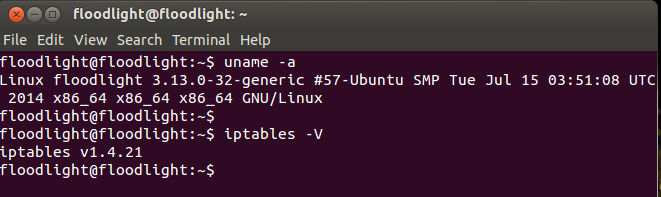
\includegraphics[width=\textwidth]{img/version.png}
\caption{Version checking}
\end{figure}

Then, we download and build the following libraries by following the installation instructions given in \cite{r2}:
\begin{itemize}
    \item libmnl-1.0.3
    \item iptables-1.4.12
    \item libnflink-1.0.0
    \item libnetfilter\_queue-1.0.2
\end{itemize}

We also install Scapy which is a python based packet crafting tool to test our implementation with a known previously known packets \cite{r3}.

\subsection{Simple Example for testing iptables}
In order to demonstrate a simple scenario about iptable rules. We configure two VMs which are shown as follows:
\begin{figure}[H]
\centering
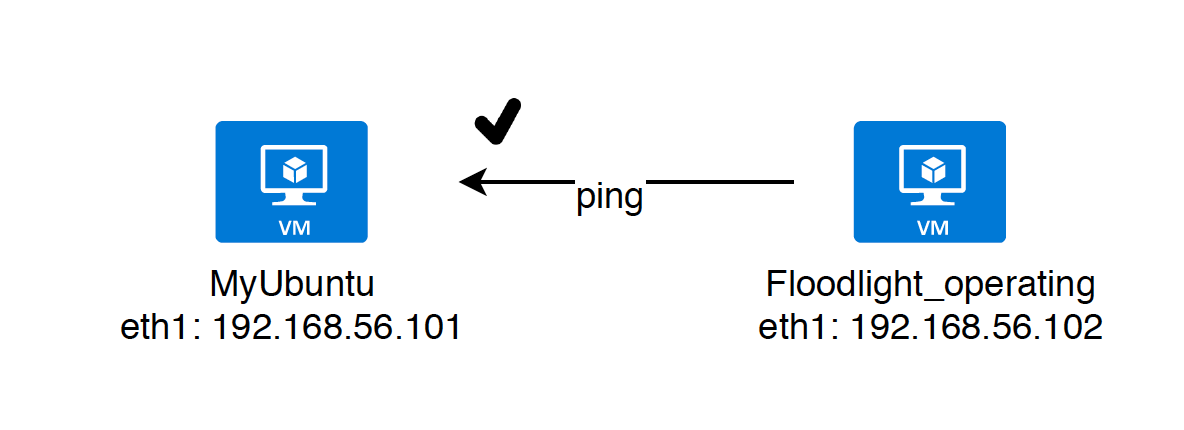
\includegraphics[width=\textwidth]{img/9.png}
\caption{Scenario 1: Successful ping}
\end{figure}

For now, both host should ping each other successfully. For that aim, we configure MyUbuntu to listen its eth1 interface via \textit{tcmpdump} tool. Then, we ping that host successfully (no drop) as shown in following figure.
\begin{figure}[H]
\centering
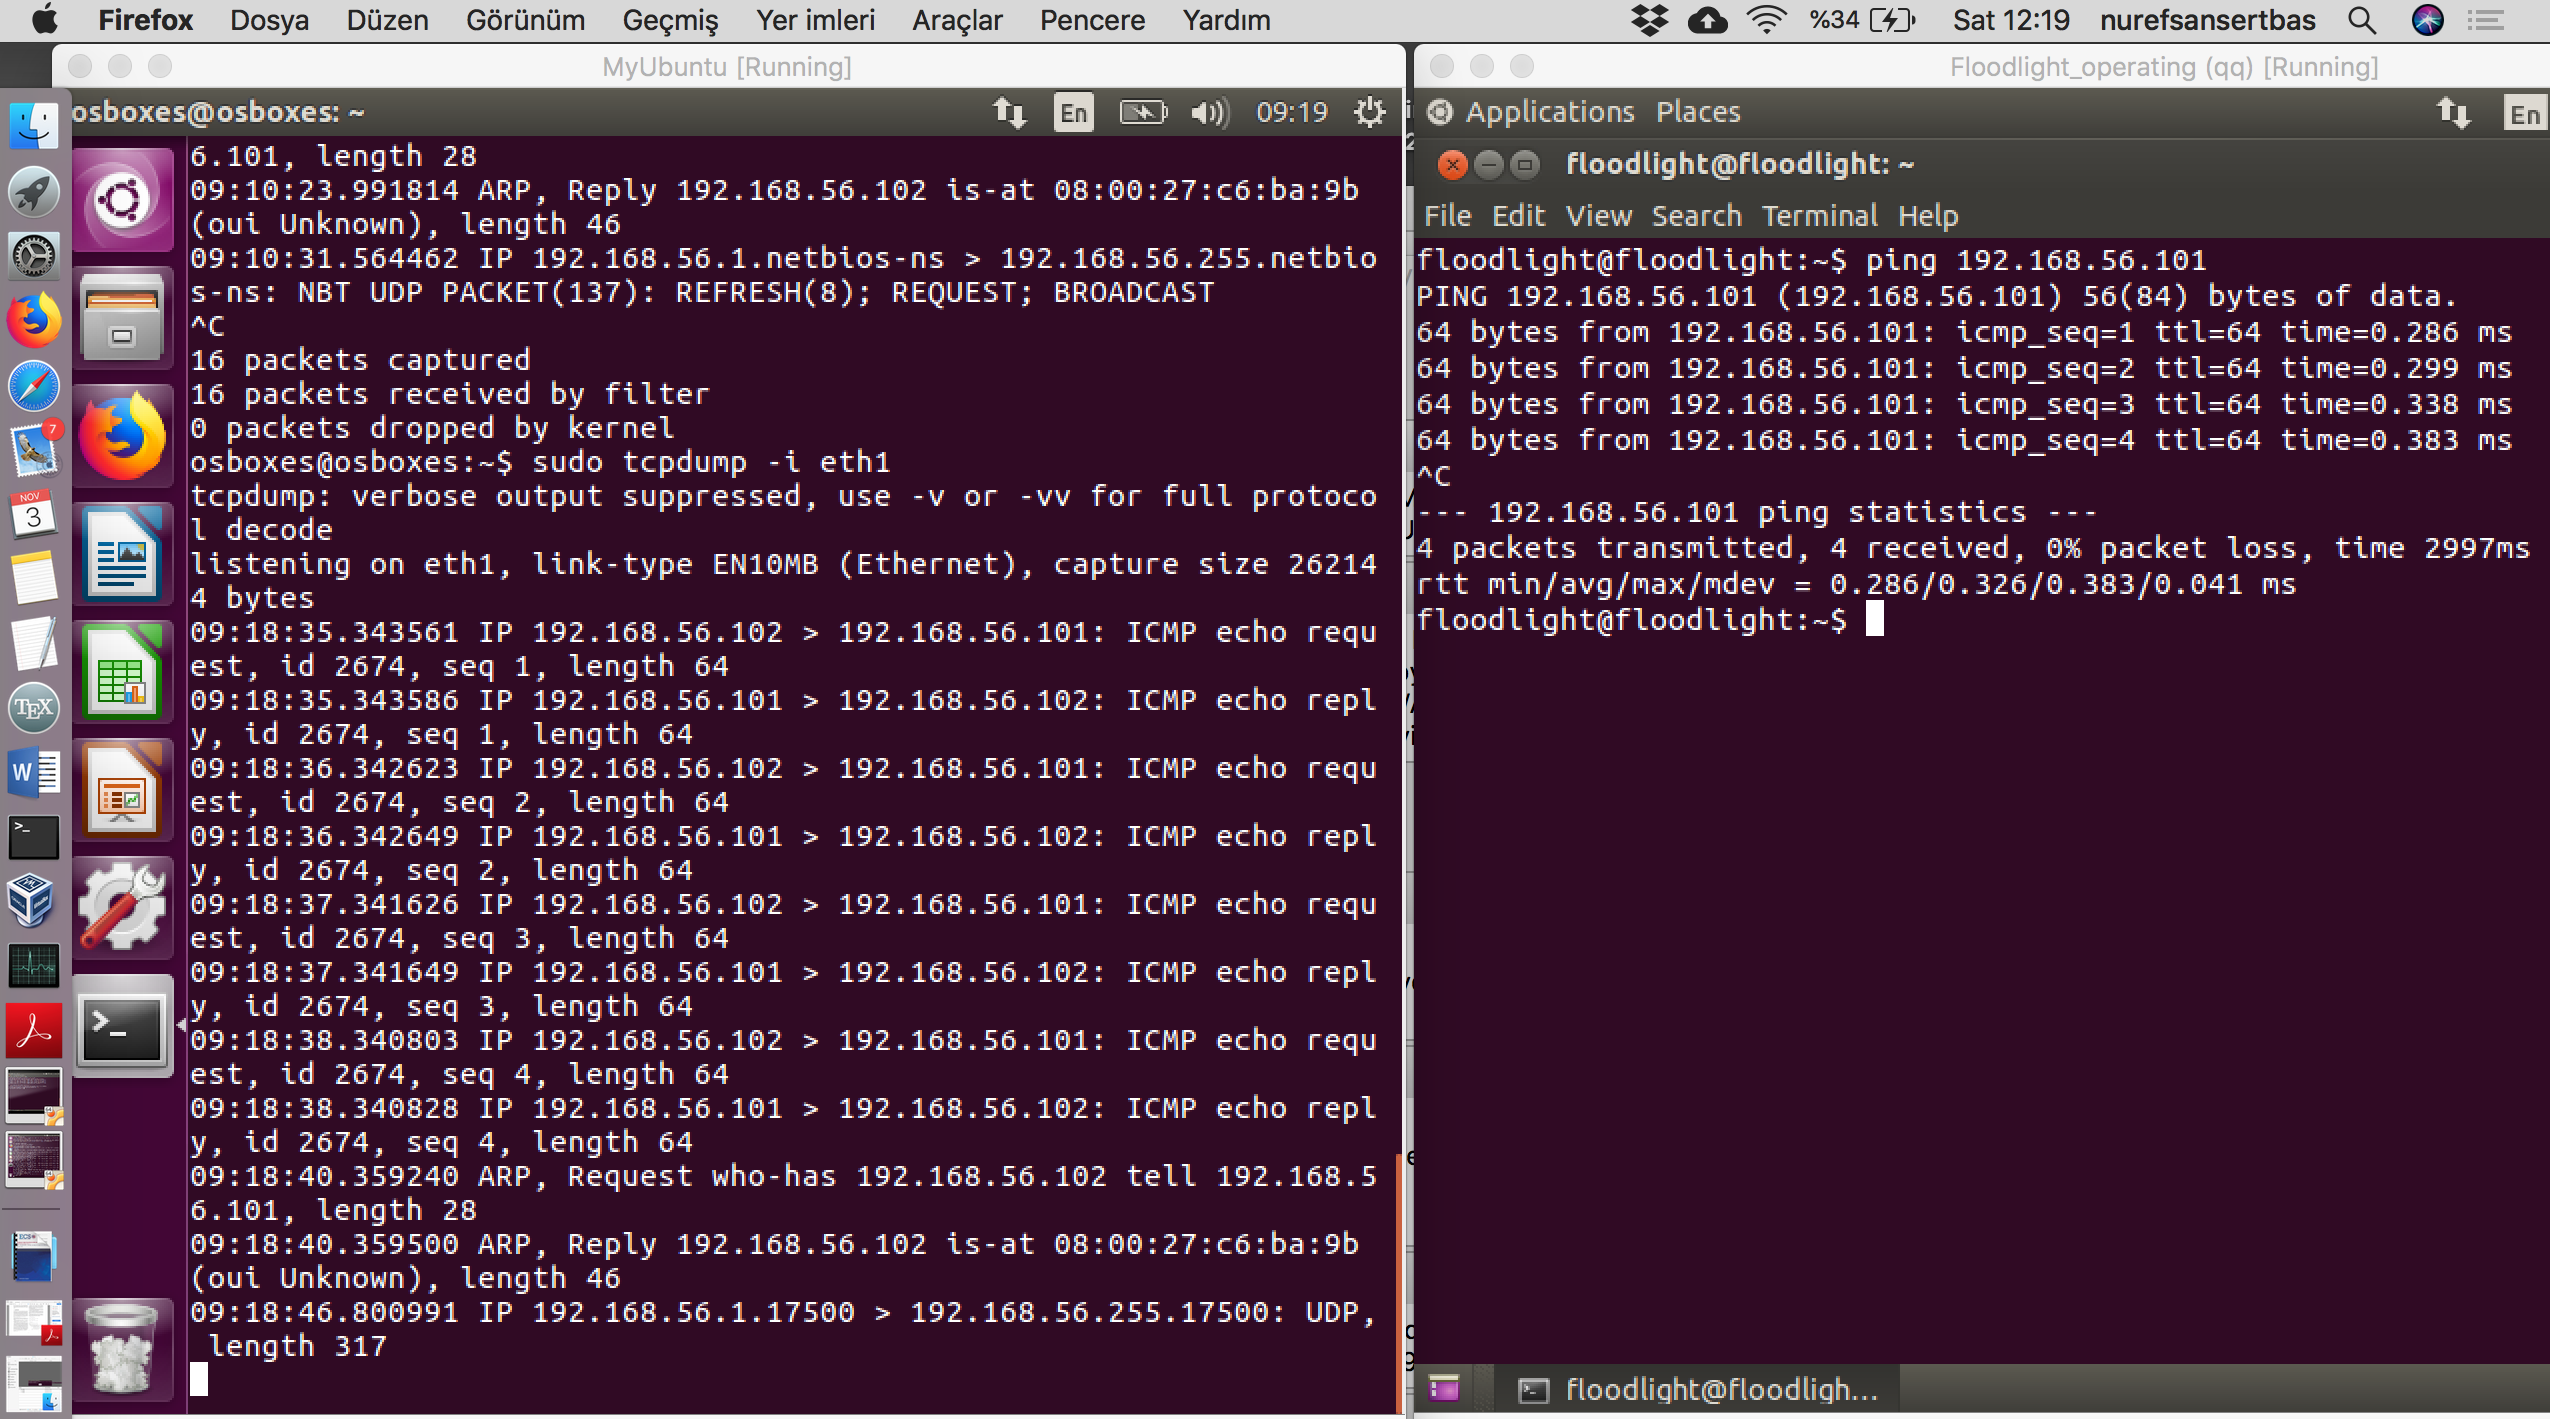
\includegraphics[width=\textwidth]{img/4.png}
\caption{Screenshot of successful ping}
\end{figure}

Now, we aim to carry out the scenario which is given in follwoing figure.

\begin{figure}[H]
\centering
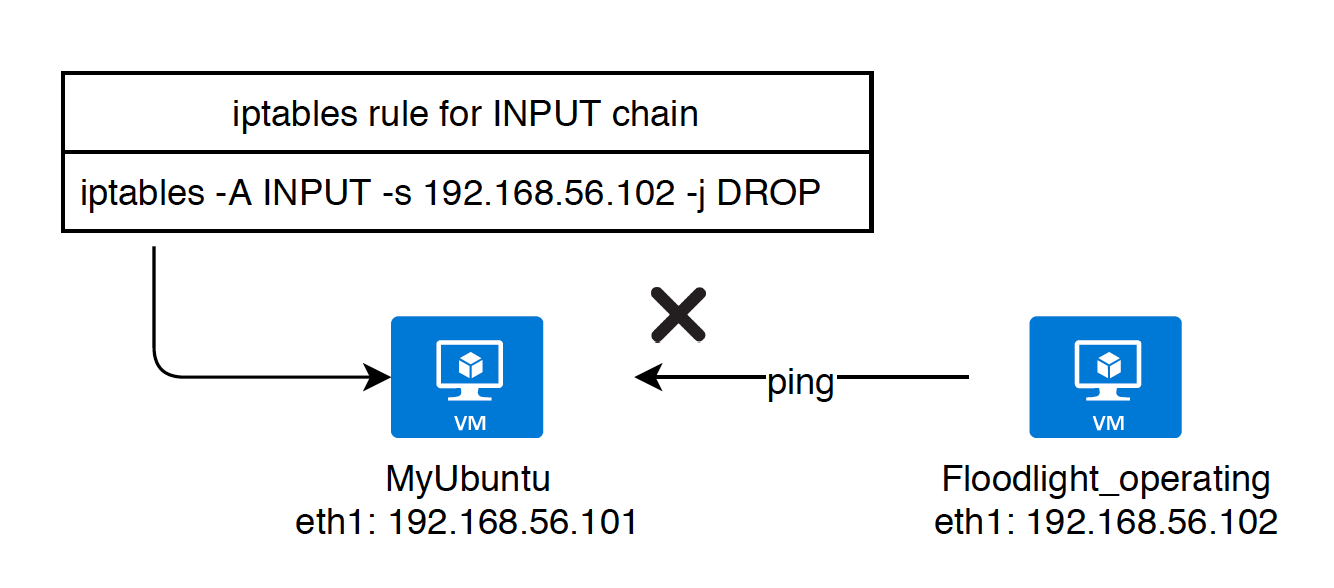
\includegraphics[width=\textwidth]{img/10.png}
\caption{Scenario 2: Failed ping}
\end{figure}

To do this, we add a drop rule into MyUbuntu for dropping packets coming from the host named Floodlight\_running whose ip is 192.168.56.102. The corresponding rule is given in following figure.
\begin{figure}[H]
\centering
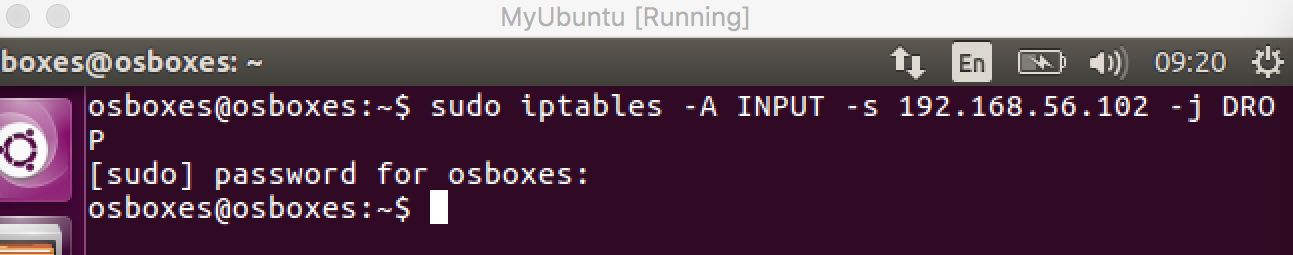
\includegraphics[width=\textwidth]{img/5.png}
\caption{Firewall rule for dropping}
\end{figure}

Then, we try to ping 192.168.56.101 again. Since we already insert drop rule for the packets coming from 192.168.56.102, we expect that the ping operating fails (See figure \ref{fail}).
\begin{figure}[H]
\centering
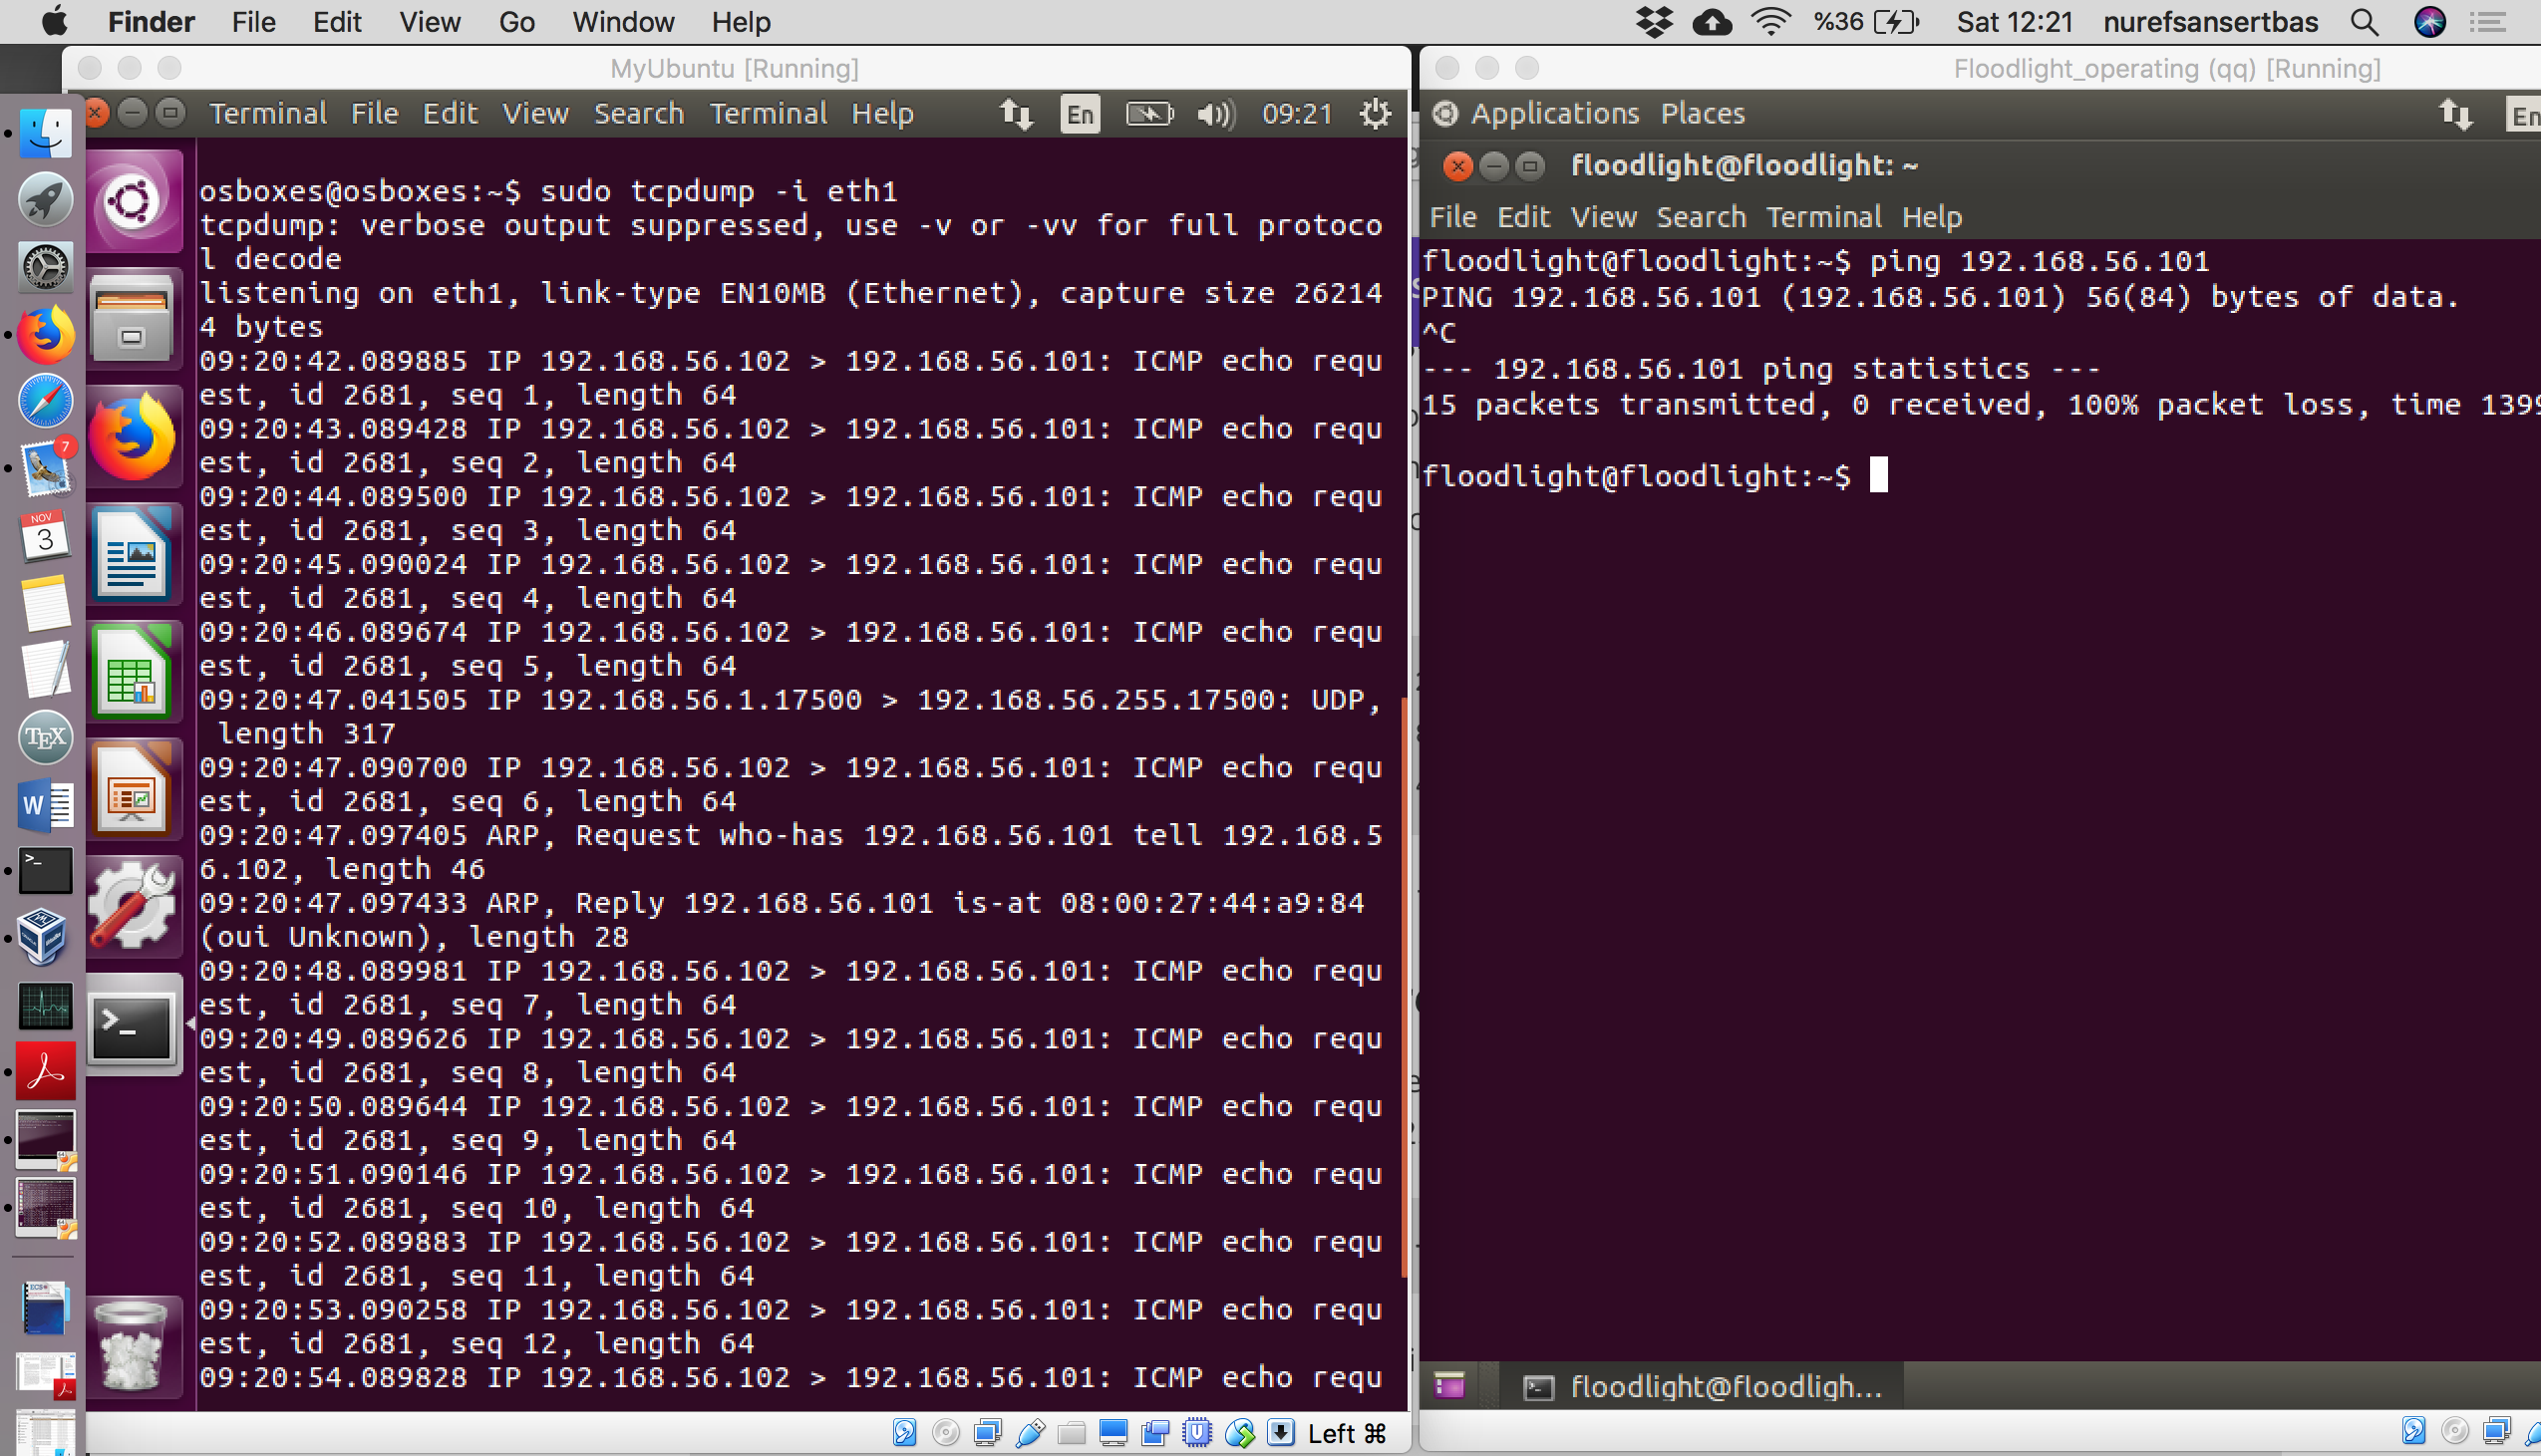
\includegraphics[width=\textwidth]{img/6.png}
\label{fail}
\caption{Screenshot of failed ping}
\end{figure}

We also check the matching statistics from the iptables as follows. It can be seen that there exist 15 matching (and dropped) packet whose source is 192.168.56.102.

\begin{figure}[H]
\centering
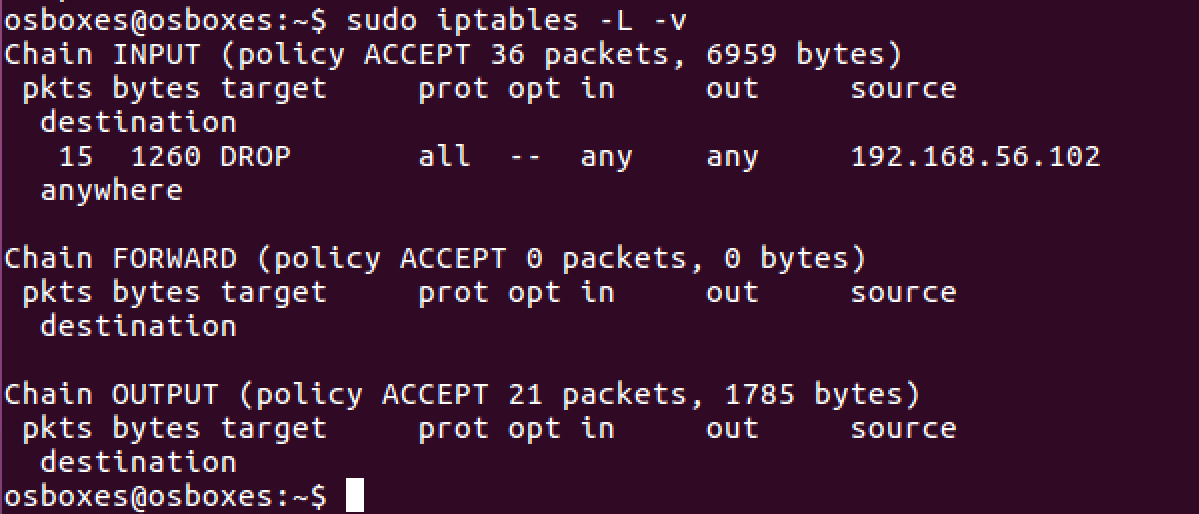
\includegraphics[width=\textwidth]{img/7.png}
\caption{Listing existing firewall rules}
\end{figure}

Finally, we clear the inserted rule into the firewall and finish the example.
\begin{figure}[H]
\centering
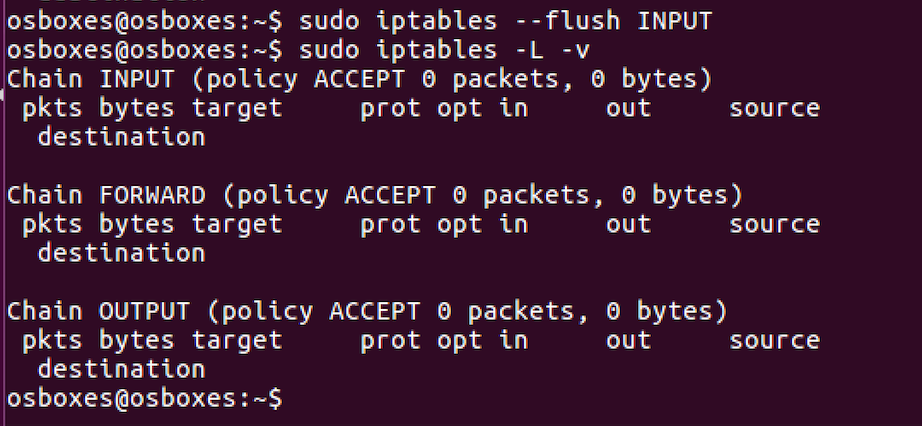
\includegraphics[width=\textwidth]{img/8.png}
\caption{Deleting firewall rules and list}
\end{figure}


\subsection{Another Example}
We also capture incoming packets through eth0 interface as given in below figure. Our aim was to capture the source port and IP addresses of the response packets (incoming packets). 
\begin{figure}[H]
\centering
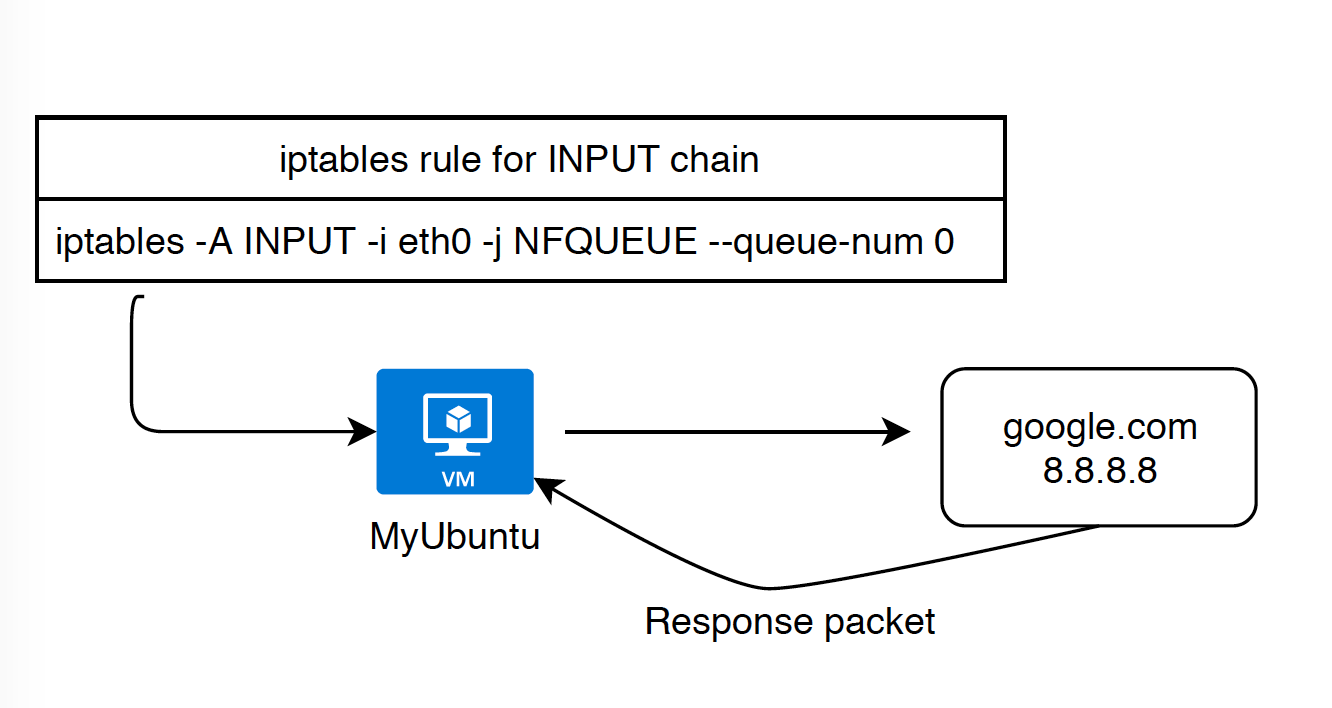
\includegraphics[width=\textwidth]{img/ex.png}
\caption{Scenario 3: Capturing eth0 interface}
\end{figure}

For that aim, we ping 8.8.8.8 and we process the captured packet headers. Then, we managed to get port and IP information from IP header.

\section{Implementation Details}
The implementation receives an input an IP address \textbf{ip}, a port \textbf{p}, a terminate packet count \textbf{i} and a string \textbf{hello}. We can divide the project work into several steps as follows:
\begin{enumerate}
    \item Reading incoming packets from the kernel queue (default NQUEUE 0): First of all, we define and add a new firewall rule for queuing the incoming packets. Then, we use \textit{libnetfiltrer\_queue} library which provides an API to packets that have been queued by the kernel packet filter. For that aim, we create a socket and bind this socket to the given queue. Then, we select \textit{copy\_packet} mode to capture the packets (line 122-160) \cite{r1}.
    \item Checking the packet headers and payload :
   The existing library function \textit{nfq\_get\_payload} provides the ip header (line 45). We use that information to parse the packet. For that aim we follow the TCP-IP stack and we obtain source IP and source port, and the app layer payload data (line 48-54). Then, we check two conditions:
   \begin{itemize}
       \item Is the source port is \textbf{p}?
       \item Is the source ip is \textbf{ip}?
   \end{itemize}
   
   In case of match (both conditions are met), we continue with the Step 3. Otherwise, we go back to Step 1 and wait for new arrivals.
    \item Further processing the payload:
    We make a sub-string search in the packet payload and we print out the appearances of the given string to the file named output.txt
    \item Returning packet back to the queue:
    In case that the number of captured packets that satisfy all conditions is equal to \textit{i}, we terminate the program by unbinding from queue and removing firewall rules.
\end{enumerate}

In order to demonstrate the output of our implementation we give a simple example. We select Floodlight VM(192.168.56.101) as a firewall host and we compile our implementation by pointing the external libraries that we have used. \\

\textbf{gcc -Wall -o cap cap.c -lnfnetlink -lnetfilter\_queue} \\

Then, we run our implementation with root privileges as follows: \\

\textbf{sudo ./cap 192.168.56.102 2000 3 hello} \\

In other words, we want to listen all incoming packets but we only capture packets whose source ip is 192.168.56.102 and source port is 2000. In case of capturing such a packet, we will check whether the packet payload contains 'hello' string or not. We also run sendPckt.py script via \textbf{sudo python sendPckt.py} command on another host to make a verification of our implementation. The command line output and the content of the output.txt file are given in following figures. 

\begin{figure}[H]
\centering
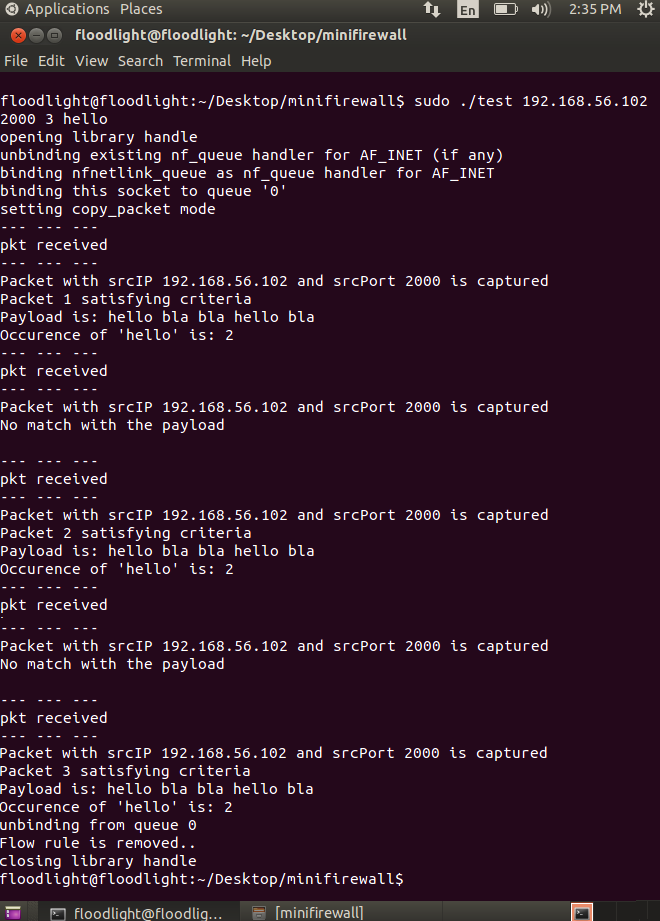
\includegraphics[width=\textwidth]{img/example.png}
\caption{Command Line Output}
\end{figure}

\begin{figure}[H]
\centering
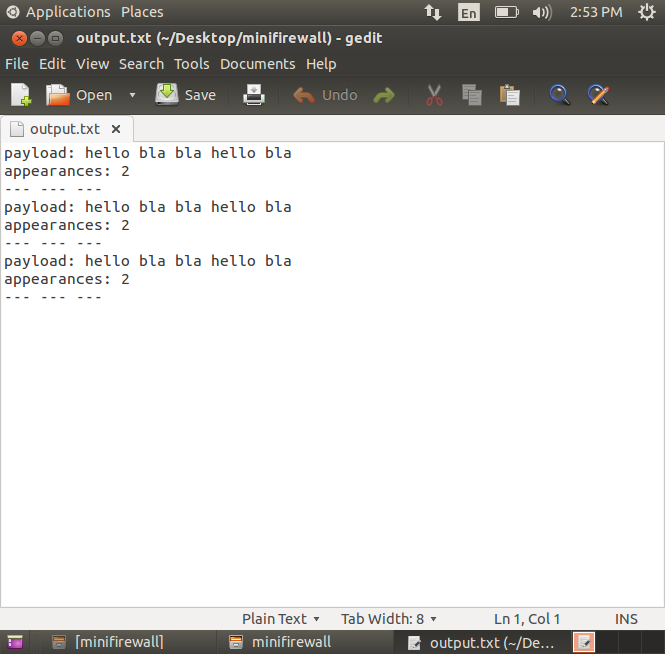
\includegraphics[width=\textwidth]{img/output.png}
\caption{Content of the output.txt file}
\end{figure}

\newpage
\section*{Additional Notes}
\begin{itemize}
\item Project code and documentation can be accessed on \url{https://github.com/sertbasn1/minifirewall.git}.
\item I preferred to use Floodlight VM which I already used for several projects. You can also download Floodlight VM from \cite{r4}.
\item In the implementation we only listen eth1 with following implicit rule '"sudo iptables -A INPUT -i eth1 -j NFQUEUE --queue-num 0"'. There is no special reason for selecting eth1 interface.
\item For the sake of simplicity, we implicitly set dest port as 2000 and dest ip as 192.168.56.101 in sendPckt.py
\end{itemize}

\printbibliography
\end{document}